\documentclass[a4paper, 12pt]{article} % тип документа

%%%Библиотеки
	%\usepackage[warn]{mathtext}	
	\usepackage[T2A]{fontenc}   %Кодировка
	\usepackage[utf8]{inputenc} %Кодировка исходного текста
	\usepackage[english, russian]{babel} %Локализация и переносы
	\usepackage{caption}
	\usepackage{listings}
	\usepackage{amsmath, amsfonts, amssymb, amsthm, mathtools}
	\usepackage[warn]{mathtext}
	\usepackage[mathscr]{eucal}
	\usepackage{wasysym}
	\usepackage{graphicx} %Вставка картинок правильная
	\DeclareGraphicsExtensions{.pdf,.png,.jpg}
	\graphicspath{ {images/} }
	
	\setlength{\parskip}{0.5cm}
	
	\usepackage{pgfplots}
	\usepackage{indentfirst}
	\usepackage{float}    %Плавающие картинки
	\usepackage{wrapfig}  %Обтекание фигур (таблиц, картинок и прочего)
	\usepackage{fancyhdr} %Загрузим пакет
	\usepackage{lscape}
	\usepackage{xcolor}
	\usepackage[normalem]{ulem}
	\usepackage{wasysym}
	
	\usepackage{titlesec}
	\titlelabel{\thetitle.\quad}

	\usepackage{hyperref}
	\newenvironment{comment}{}{}

%%%Конец библиотек

%%%Настройка ссылок
	\hypersetup
	{
		colorlinks = true,
		linkcolor  = blue,
		filecolor  = magenta,
		urlcolor   = blue
	}
%%%Конец настройки ссылок


%%%Настройка колонтитулы
	\pagestyle{fancy}
	\fancyhead{}
	\fancyhead[L]{2.4.1}
	\fancyhead[R]{Старченко Иван, группа Б01-005}
	\fancyfoot[C]{\thepage}
%%%конец настройки колонтитулы

\begin{document}

\begin{center}
  \LARGE{Лабораторная работа 3.1.3}\\[0.2cm]
  \LARGE{Иследование магнитного поля Земли.}\\[0.2cm]
  \large{25 сентября 2021 г.}\\[0.2cm]
  \large{Старченко Иван Александрович}\\[0.2cm]
\end{center}

\textbf{Цель работы:}  исследовать свойства постоянных неодимовых магнитов;
измерить с их помощью горизонтальную и вертикальную составляющие
индукции магнитного поля Земли и магнитное наклонение.
\\

\textbf{Оборудование:} неодимовые магниты; тонкая нить для изготовления крутильного маятника; медная проволока; электронные весы; секундомер; измеритель магнитной индукции; штангенциркуль; брусок, линейка
и штатив из немагнитных материалов; набор гирь и разновесов.

\section{Теория}
\begin{enumerate}
    \item 


 Простейший магнитный диполь может быть образован витком с током или постоянным магнитом. По определению, магнитный момент \textbf{m}
тонкого витка площадью S с током I равен (в системе СИ)
\begin{equation}
    \textbf{m}=I\textbf{S},
    \label{eq:m}
\end{equation}
где \textbf{S} = S\textbf{n} — вектор площади контура, образующий с направлением тока правовинтовую систему, \textbf{n} — единичный вектор нормали к площадке
(это же направление m принимается за направление S →N от южного S к северному N полюсу магнита). Если размеры контура с током
или магнитной стрелки малы по сравнению с расстоянием до диполя, то
соответствующий магнитный диполь m называют элементарным, или
точечным.

Магнитное поле точечного диполя определяется по формуле, аналогичной формуле для поля элементарного электрического диполя:
\begin{equation}
    \textbf{B}_{дип}=\frac{\mu_0}{4\pi} \left(\frac{3(\textbf{m, r})\textbf{r}}{r^5}-\frac{\textbf{m}}{r^3} \right)
    \label{eq:Bdip}
\end{equation}

Во внешнем магнитном поле с индукцией \textbf{B} на точечный магнитный
диполь m действует механический момент сил
\begin{equation}
    \textbf{M}=[\textbf{m},\textbf{B}].
    \label{eq:M}
\end{equation}
При этом потенциальная энергия, которой обладает диполь с постоянным \textbf{m}, равна
\begin{equation}
    W=-(\textbf{m,B})
    \label{eq:W}
\end{equation}
В неоднородном внешнем поле выражение для энергии постоянного
диполя (\ref{eq:W}) сохраняется. При этом кроме момента сил на диполь действует ещё и сила
\begin{equation}
    \textbf{F}=-\nabla W= (\textbf{m},\nabla)\textbf{B}.
    \label{eq:F}
\end{equation}

Выражения (\ref{eq:Bdip}) и (\ref{eq:F}) позволяют рассчитать силу взаимодействия магнитов с моментами $\textbf{m}_1$ и $\textbf{m}_2$ в рамках модели точечных диполей. В частном случае, когда моменты двух небольших магнитов направлены вдоль соединяющей их прямой: $\textbf{m}_{1,2}$ || \textbf{r}, где \textbf{r} — радиус-вектор между ними, магниты взаимодействуют с силой
\begin{equation}
    F_{1,2}=\textbf{m}_1\frac{\partial B_2}{\partial r}=-\frac{\mu_0}{4\pi}\frac{6m_1m_2}{r^4}.
    \label{eq:F||}
\end{equation}

Если магнитные моменты направлены перпендикулярно соединяющей их прямой: $\textbf{m}_{1,2}$ $\bot$ \textbf{r}, то нетрудно показать, что сила их взаимодействия окажется в два раза меньшей и будет иметь противоположный
знак:
\begin{equation}
    F_{1,2}=\frac{\mu_0}{4\pi}\frac{3m_1m_2}{r^4}.
    \label{eq:Fbot}
\end{equation}


\item
Магнитное поле однородно намагниченного шара радиусом R может
быть вычислено точно. На расстояниях $r\geq R$ от центра шара оно совпадает с полем точечного магнитного диполя (\ref{eq:Bdip}), расположенного в центре, магнитный момент \textbf{m} которого совпадает с полным моментом шара.
Внутри шара магнитное поле однородно: c помощью формулы (\ref{eq:Bdip}) и условия непрерывности нормальной компоненты индукции на поверхности
шара нетрудно получить, что при r < R
\begin{equation}
    \textbf{B}_0=\frac{\mu_0\textbf{m}}{2\pi R^3}.
    \label{eq:B0}
\end{equation}

В качестве ещё одной характеристики материала магнита используют остаточную намагниченность $\textbf{M}$. По определению, намагниченность равна объёмной плотности магнитного момента, поэтому для однородно намагниченного шара
\begin{equation}
    \textbf{m}=\textbf{M}V,
\end{equation}
где $V=\frac{4\pi R^3}{3}$ - объем магнита. Величину $\textbf{B}_r=\mu_0 \textbf{M}$ называют остаточной индукцией материала.

Из (\ref{eq:Bdip}) нетрудно видеть, что индукция $\textbf{B}_p$ на полюсах однородно намагниченного шара направлена по нормали к поверхности и совпадает
поэтому с индукцией внутри шара $\textbf{B}_p=\textbf{B}_0$. Как следует из (\ref{eq:B0}), величина $B_p$ связана с остаточной индукцией $B_r$ соотношением
\begin{equation}
    B_p=B_0=\frac{2}{3}B_r.
\end{equation}
\end{enumerate}

\section{Измерение магнитного момента магнитных шариков}
\begin{wrapfigure}{r}{0.25\linewidth}
    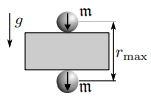
\includegraphics[width=\linewidth]{methodA.png}
    \caption{Измерение магнитных моментов шариков}
    \label{fig:methodA}
\end{wrapfigure}
\textbf{Метод А}.
Величину магнитного момента m двух
одинаковых шариков можно рассчитать, зная их
массу m и определив максимальное расстояние $r_{max}$
на котором они ещё удерживают друг друга в поле
тяжести (Рис.\ref{fig:methodA} ). При максимальном расстоянии
сила тяжести шариков mg равна силе их магнитного
притяжения.
Когда векторы двух магнитных моментов ориентированы вертикально, из (\ref{eq:F||}) имеем
\begin{equation}
    m=\sqrt{\frac{2\pi m'gr^4_{max}}{3\mu_0}}.
    \label{eq:mA}
\end{equation}
По величине m с помощью (\ref{eq:Bdip}) можно рассчитать величину индукции \textbf{B} вблизи любой точки на поверхности шара радиуса R. Максимальная величина индукции наблюдается на полюса.

\begin{wrapfigure}{r}{0.3\linewidth}
    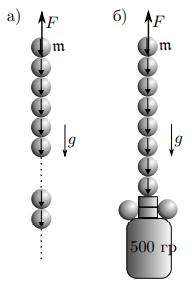
\includegraphics[width=\linewidth]{methodB.png}
    \caption{Альтернативный метод измерения магнитных моментов шариков}
    \label{fig:methodB}
\end{wrapfigure}
\textbf{Метод Б}. Величину магнитного момента шариков можно определить также по силе их сцепления. Она определяется как сила, необходимая для разрыва двух сцепившихся магнитных шариков. Сила сцепления
максимальна, если шары соединяются своими противоположными полюсами (магнитные моменты сонаправлены).
Максимальную силу сцепления можно
определить по весу магнитной цепочки, которую способен удержать самый верхний магнитный шарик. Если цепь состоит из одинаковых магнитных шариков (Рис. \ref{fig:methodB}), то
при определённой длине она отрывается от
верхнего шарика. При этом, учитывая, что
сила притяжения убывает как $F\propto 1/r^4$, где
r — расстояния между центрами шаров, для
расчёта прочности цепочки достаточно учитывать силу взаимодействия верхнего шара
с 3–4 ближайшими соседями.

Сила сцепления (\ref{eq:F||}) двух одинаковых шаров радиусами R c магнитными моментами m равна
\begin{equation}
    F_0=\frac{\mu_0}{4 \pi}\frac{3m^2}{8R^4}.
    \label{eq:F0}
\end{equation}
Тогда минимальный вес цепочки, при которой она оторвётся от верхнего
шарика, равен
\begin{equation}
    F=F_0\left(1+\frac{1}{2^4}+\frac{1}{3^4}+\frac{1}{4^4}+...\right)\approx1,08F_0.
    \label{eq:1,08F0}
\end{equation}

\section{Измерение горизонтальной составляющей индукции магнитного
поля Земли}

Магнитное поле Земли в настоящей работе измеряется по периоду
крутильных колебаний «магнитной стрелки» вокруг вертикальной оси.
\begin{wrapfigure}{r}{0.3\linewidth}
    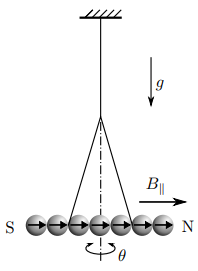
\includegraphics[width=\linewidth]{B||.png}
    \caption{Крутильный майтник во внешнем магнитном поле}
    \label{fig:B||}
\end{wrapfigure}

«Магнитная стрелка» образована сцепленными друг с другом n намагниченными
шариками. С помощью $\wedge$-образного подвеса
стрелка подвешена в горизонтальном положении (Рис. \ref{fig:B||}). Для крепления нити в
работе используется штатив, изготовленный
из немагнитного материала.

Магнитные моменты всех шариков направлены в одну сторону вдоль оси «стрелки». Под действием механического момента
сил (\ref{eq:M}), действующего на стрелку со стороны
поля Земли, стрелка стремится повернуться
по горизонтальной составляющей магнитного поля Земли $\textbf{B}_{||}$ в направлении Юг—Север.

При отклонении стрелки на угол $\theta$ от равновесного положения в горизонтальной плоскости возникают крутильные колебания вокруг вертикальной оси, проходящей через середину стрелки. Если пренебречь упругостью нити, то уравнение крутильных колебаний такого
маятника определяется возвращающим моментом сил
\begin{equation}
    \mathcal{M}=-m_nB_{||}\sin\theta
\end{equation}
и моментом инерции $J_n$ «стрелки» относительно оси вращения. При малых амплитудах ($sin \theta \approx \theta$) уравнение колебаний стрелки имеет вид
\begin{equation}
    J_n\ddot{\theta}+m_nB_{||}\theta=0.
\end{equation}
Отсюда находим период малых колебаний:
\begin{equation}
    T=2\pi \sqrt{\frac{J_n}{m_nB_{||}}}.
\end{equation}

Здесь $m_n$ = nm — полный магнитный момент магнитной «стрелки»,
составленной из n шариков. Момент инерции $J_n$ стрелки из n шариков с
хорошей точностью равен моменту инерции тонкого однородного стержня массой $m_n'$ = nm' и длиной $l_n$ = 2nR:
\begin{equation}
    J_n\approx\frac{m_n'l_n}{12}=\frac{n^3m'R^2}{3}.
\end{equation}
Отсюда находим, что период колебаний маятника пропорционален числу
шаров n, составляющих «стрелку»:
\begin{equation}
    T_n=2\pi\sqrt{\frac{m'R^2}{3mB_{||}}}\cdot n.
    \label{eq:Tn}
\end{equation}

\section{Измерение вертикальной составляющей индукции магнитного поля
Земли. Магнитное наклонение}

Для измерения вертикальной $B_{\bot}$ составляющей вектора индукции
поля Земли используется та же установка, что и для измерения горизонтальной составляющей с тем лишь отличием, что подвешенная магнитная «стрелка» закрепляется на нити в одной точке. В этом случае
стрелка, составленная из чётного числа одинаковых шариков и подвешенная за середину, расположится не горизонтально, а под некоторым
углом к горизонту (Рис. \ref{fig:Bbot}).
\begin{figure}[h!]
    \centering
    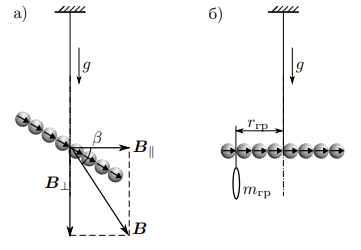
\includegraphics[width=8cm]{Bbot.png}
    \caption{Измерение вертикальной составляющей поля и магнитного наклонения}
    \label{fig:Bbot}
\end{figure}
Это связано с тем, что вектор \textbf{B} индукции магнитного поля Земли не горизонтален, а образует с горизонтом
некоторый угол $\beta$, зависящий от географической широты $\phi$ места, где
проводится опыт. Величина угла $\beta$ называется магнитным наклонением.

Измерить магнитное наклонение непосредственно по положению подвешенной «стрелки» затруднительно из-за механического момента нити
в точке подвеса, неизбежно возникающем при наклоне «стрелки». Избавиться от этого можно, если выровнять её горизонтально с помощью
небольшого дополнительного грузика (Рис. \ref{fig:Bbot}б). В этом случае момент силы тяжести груза относительно точки подвеса будет равен моменту сил, действующих на «стрелку» со стороны вертикальной составляющей магнитного поля Земли. Если масса уравновешивающего груза равна $m_{гр}$, плечо силы тяжести $r_{гр}$, а полный магнитный момент стрелки $m_n$ = nm, то в равновесии
\begin{equation}
    \mathcal{M}_n=m_{гр}gr_{гр}=nmB_\bot.
\end{equation}
\section{Ход работы}
\begin{enumerate}
    \item 

Измерим массу и диаметр магнитных шариков, для этого взвесим на весах N=30 и линейкой измерим длину цепи, составленной из этих шариков. $m_N=(25,231\pm0,001)г\Rightarrow m=\frac{m_N}{N}=(0,841\pm0,001)г$; $l_N=(17,70\pm0,05)см\Rightarrow d=\frac{l_N}{N}=(0,59\pm0,05)см$.
С помощью магнитометра измерим индукции поля на полюсах шарика: $B_p=258\ мТл$. 

\item Определим величину магнитного момента шарика m по методу А. Для этого измерим максимальную толщину пластинки, через которую шарики еще удерживаются в поле тяжести. $h_{max}=(19,0\pm0,1)мм$. Используя формулу (\ref{eq:mA}) получаем $m=(72\pm7)\cdot 10^{-3}\ A\cdot м^2$. Отсюда можно найти значения для намагничености, остаточной индукции и индукции магнитного поля на полюсе шарика: $M=\frac{m}{V}=(64\pm5)\cdot 10^{4}\ A/м$, $B_r=0,467\pm0,05\ Тл$, $B_p=\frac{2}{3}B_r=0,325\pm0,03\ Тл$, что расходится с измерениями по магнитометру. Эти расхождения могут быть связаны с трудностью точного измерения магнитометром из-за малых размеров магнита.
\item Определим величину магнитного момента шарика m по методу Б. Для этого составим цепь из 29 магнитов и дополнительных грузов, которые будем присоединять пока вся система не будет отпадать от верхнего магнита. Это произшло при массе системы $m_{кр}=212,699\ г$, тогда, пользуясь формулами (\ref{eq:F0}) и (\ref{eq:1,08F0}), получим, что $m=\sqrt{\frac{800m_{кр}g\pi R^4}{81\mu_0}}\Rightarrow m=(79\pm 8)\cdot10^{-3}\ A\cdot м^3$. Аналогично методу А найдем необхожимые величины: $M=\frac{m}{V}=(71\pm14)\cdot 10^{4}\ A/м$, $B_r=0,496\pm0,8\ Тл$, $B_p=\frac{2}{3}B_r=0,341\pm0,5\ Тл$, что хорошо сходится с методом А, но плохо сходится с измерениями магнитометра.

Заметим, что в обоих методах остаточная индукция 1,5 раза отличается от табличного значения. 
\item
Соберем куртильный маятник из 12 магнитных шариков. Сначала сформируем из них кольцо и убедимся, что упругость нитки не влияет на колебания. 
\begin{figure}[h!]
    \centering
    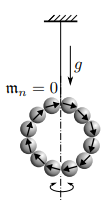
\includegraphics[]{circle.png}
    \caption{Крутильный майтник во внешнем магнитном поле}
\end{figure}

Теперь сформируем магнитную "стрелку" и возбуждая крутильные колебания найдем зависимость периода колебаний от количества магнитов в "стрелке". Приведем значения в таблице.
\newpage
\begin{table}
\centering
\begin{tabular}{|l|l|l|l|l|l|l|l|l|l|l|}
\hline
$n$ & 12    & 11    & 10    & 9     & 8     & 7     & 6     & 5     & 4     & 3    \\ \hline
$T$, с & 5.594 & 5.146 & 4.552 & 4.081 & 3.827 & 3.263 & 2.823 & 2.243 & 1.773 & 1.156 \\ \hline
\end{tabular}
\caption{Зависимость периода колебаний крутильного маятника от количества магнитов в "стрелке"}
\end{table}
Зная коэффициент наклона прямой мы можем найти значение горизонтальной составялющей магнитного поля Земли по формуле (\ref{eq:Tn}). $k=2\pi \sqrt{\frac{m'R^2}{3mB_{||}}}$, где m' - масса одного шарика. Значит $B_{||}^{-1}=\frac{3mk^2}{4\pi^2 m'R^2}$.
\begin{figure}[H]
    \centering
    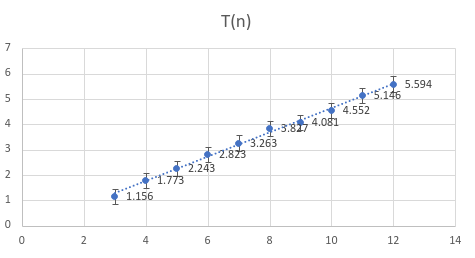
\includegraphics{T(n).png}
    \caption{Зависимость периода колебаний T от количества магнитов n в "стрелке"}
\end{figure}

Из метода нименьших квадратов находим $k=0,4814\pm0,0043\Rightarrow B_{||}=(18\pm1)\ мкТл$. 
\item Определим вертикальную составляющую магнитного поля Земли с помощью той же магнитной "стрелки", которую будем составлять из четного числа шариков и подвешивать за середину. Уравновешивая конструкцию с помощью кусочков проволоки найдем механически момент, который дествует на "стрелку", в зависимости от количества магнитов в "стрелке". Результаты приведем в таблице:
\begin{table}[h!]
\centering
\begin{tabular}{|c|c|c|c|c|c|}
\hline
M, $\cdot 10^{-7} н\cdot м$ & 28,32 & 21,24 & 14,16 & 7,08 & 1,80 \\ \hline
n                       & 12    & 10    & 8     & 6     & 4    \\ \hline
\end{tabular}
\caption{Зависимость момента, действующего на "стрелку", от количества магнитов.}
\end{table}

Угловой коэффициент наклона графика будет равен $k=mB_{\bot}$.
\begin{figure}[H]
    \centering
    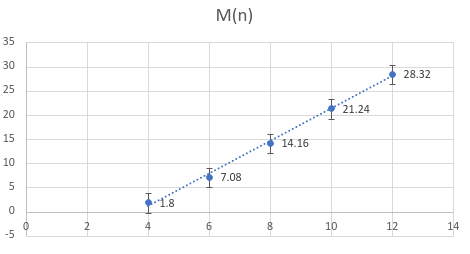
\includegraphics{M(n).png}
    \caption{Зависимость момента M, действующего на "стрелку", от количества магнитов n.}
\end{figure}

Из метода наименьших квадратов находим $k=3,36\cdot 10^{-6}\Rightarrow B_\bot=46\pm7\ мкТл$.

Найдем магнитное наклонение: $tg\beta=\frac{B_\bot}{B_{||}}\Rightarrow \beta=69^{\circ}\pm4^{\circ}$. А полное магнитное поле Земли равно $B=\sqrt{B_\bot^2+B_{||}^2}=49\pm6\ мкТл$.

\section{{Вывод}}


Мы исследовали свойства постоянных неодимовых магнитов;
измерили с их помощью горизонтальную и вертикальную составляющие
индукции магнитного поля Земли и магнитное наклонение.


\section{{Список используемой литературы}}

$\bullet$ \href{https://vk.com/doc-139677307_612194888}{Никулин М.Г. Лабораторный практикум по общей физике. Электричество и магнетизм}\\

$\bullet$ \href{https://mipt.ru/education/chair/physics/S_III/lab_el.php}{Описание лабораторных работ на кафедре общей физики МФТИ}

$\bullet$ \href{https://vk.com/doc-139677307_612194961}{П.В. Попов, А.А. Нозик. Обработка результатов учебного эксперимента}


\end{enumerate}
\end{document}
